\chapter{Software Requirements Specification}
	Das Software Requirements Specification, kurz SRS, ist ein veröffentlichter Standard zur Spezifikation einer Software. Der Inhalt eines SRS ist vom Institute of Electrical and Electronics Engineers im Standard IEEE 830-1998 festgehalten.
	
	Die Aufbau dieses Kapitels entspricht der Struktur, die in dem Standard beschriebenen wird. Einige Kapitel des SRS werden allerdings nicht behandelt, da sie keine Relevanz für NoRPG haben oder an einer anderer Stelle in diesem Dokument auftauchen.
	
\section{Einführung}
	Das erste Kapitel des SRS enthält eine Beschreibung und eine Übersicht über alles, was im SRS enthalten ist.
	
	\subsection{Zweck}
		Das SRS beschreibt den kompletten Projektumfang und die Anforderungen an die Software NoRPG. Es illustriert den Zweck und die vollständige Erklärung für die Entwicklung der Software. Dabei werden unter anderem Systemeinschränkungen, Schnittstellen und Interaktionen mit externen Schnittstellen thematisiert\footnote{vgl. Tripp \cite{srsIEEE}(1998) Seite 3}. 
	
		Die Zielgruppe des SRS bzw. die Stakeholder des Projektes sind alle Personen und Personengruppen, die in irgendeiner Verbindung mit NoRPG stehen oder jene, die Interesse an der Umsetzung haben\footnote{vgl. Rozanski \cite{rozanski2011}(2011) Seite 6}. Zudem dient die Spezifikation zur Kommunikation zwischen den Stakeholdern und den Entwicklern.
		
	\subsection{Umfang}
		Dieses SRS handelt von der in Kapitel 2 beschrieben Software NoRPG. 
		
\section{Allgemeine Beschreibung}
	Im zweiten Kapitel des SRS werden allgemeinen Faktoren, die das Produkt und seine Anforderungen betreffen, beschrieben. Dieses Kapitel bietet einen Überblick über die Systemfunktionalitäten und stellt verschiedene Arten von Stakeholdern und deren Interaktionen mit dem System vor. Dieses Kapitel behandelt jedoch nicht die spezifischen Anforderungen, sondern stellt den Hintergrund für diese dar. 

	\subsection{Produktperspektive}
		Das zu beschreibende vollständige System NoRPG besteht aus mehreren Komponenten, die auf unterschiedlichsten weisen mit den Stakeholdern kommunizieren. Daher ist es besonders wichtig, das Produkt in unterschiedlichen Perspektiven mit verwandten und geplanten Produkten zu betrachten. Aus diesem Grund werden alle System-, Benutzer-, Hardware- und Softwareschnittstellen von NoRPG betrachtet. 
		
		Folgende Grafik stellt dabei die High-Level-View von NoRPG und seinen Komponenten dar. Die Grafik stellt alle Schnittstellen zwischen NoRPG und mit anderen Produkten dar.
		
		\begin{center}
			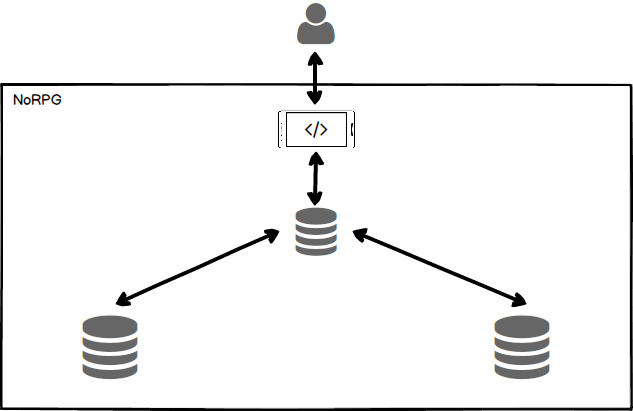
\includegraphics[width=12cm]{pics/HighLevelView.png}
			\captionof{figure}{High-Level-View von NoRPG} 
		\end{center}
		
		Das vollständige System von NoRPG besteht aus zwei Kernkomponenten. Die erste Kernkomponente ist die Android App, welche sich aus dem Quellcode des Spieles und einer eingebetteten lokalen Datenbank zusammensetzt. Die zweite Kernkomponente ist eine Datenbank, die sich auf einem Server befindet.
		
		Die Schnittstelle zwischen der App und dem Betriebssystem Android ist eine Systemschnittstelle. Systemschnittstellen identifizieren die Funktionalität der Software, um die Systemanforderung und Schnittstellenbeschreibung zu erfüllen, damit die Software mit dem System übereinstimmt\footnote{vgl. Tripp \cite{srsIEEE}(1998) Seite 13}.
		
		Bei der App von NoRPG handelt es sich um die Benutzerschnittstelle des Systems. Benutzerschnittstellen beschreiben die Kommunikation zwischen NoRPG und dem User. Die Benutzeroberfläche der App ist die einzige Möglichkeit für den Anwender mit dem System zu interagieren.
		
		Jede Schnittstelle zwischen NoRPG und Hardwarekomponenten des Systems werden als Hardwareschnittstellen bezeichnet. Das Smartphone mit all seinen Komponenten sind einzige Hardwarekomponente, zu der eine direkte  Schnittstelle existiert. Die Hardwarekomponenten eines Smartphones sind das Touchscreen, die Lautsprecher oder der WLAN-Adapter. Diese Komponenten werden in der Abbildung durch das Smartphone zusammengefasst.
		
		Die App kommuniziert mit der lokalen sowie mit der serverseitigen Datenbank. Dabei handelt es sich um Softwareschnittstellen. Sie bilden den Übergang zwischen unterschiedlichen Programmen und ermöglichen dadurch das Nutzen derer Funktionalitäten. 

	\subsection{Produktfunktionen}
		In diesem Unterkapitel werden die wichtigsten Funktionen von NoRPG zusammengefasst. Wie in Kapitel 2 beschrieben ist das Hauptziel von NoRPG Lernspiele in einer standardisierten Reihenfolge zum Herunterladen anzubieten. Dieses Ziel macht das Downloaden von Spielen zu der Hauptfunktionalität von NoRPG. 
		
		Neben dieser Funktion gibt es allerdings weitere Produktfunktionen, um NoRPG attraktiver zu gestalten und um NoRPG zu personalisieren. Der Spieler wird in der Lage sein mit Elementen im Spiel zu interagieren und dabei Spielgegenstände zu sammeln. Um dem Anwender eindeutig identifizieren zu können, wird NoRPG über eine eigene Anmelde- und Registrierungsfunktion verfügen. In diesem Registrierungsprozess ist es dem Spieler möglich, seinen eigenen persönlichen Charakter zu erstellen.
		
		Im Spiel selbst wird es neben Spieloptionen wie Qualitäts- und Audioeinstellungen noch Features geben, die das Spielerlebnis verbessern sollen. Der User wird in der Lage sein eine Karte von der Spielwelt zu öffnen, eine Liste von allen herunterladbaren Spielen zu verwalten und seinen Fortschritt zu betrachten.
		
		Die App speichert den Fortschritt und die Daten in der lokalen eingebetteten Datenbank und synchronisiert diese Informationen mit der Datenbank auf dem Server.
	
	\subsection{Benutzermerkmale}
		Im Rahmen dieser Studienarbeit wird zunächst nur eine Benutzergruppe vollständig implementiert.
		
		Die zu implementierende Benutzergruppe sind die User, viel mehr die Spieler. Grundsätzlich richtet sich NoRPG an Kinder, die keine Möglichkeit haben eine Schule zu besuchen. Jedoch werden keine Benutzergruppen für diese App ausgeschlossen. Egal ob jung oder alt, männlich oder weiblich, er Spieler sollte nur eine Neugier zum Lernen mitbringen. 
		
		Der Spieler benötigt Erfahrung mit der Verwendung eines Smartphones, insbesondere mit einem Android-Systems. Dazu zählt die Bedienung der Android-Oberfläche und die des Google Play Stores. Zudem sollten die User englische Texte verstehen können, da NoRPG zunächst nur in der englischen Sprache erscheinen wird.
			
	\subsection{Einschränkungen}
		Es wird zwischen Einschränkungen für Entwickler und für Spieler unterschieden.
		
		Grundsätzlich müssen Entwickler sich an die regulatorischen Richtlinien, wie beispielsweise an die Datenschutzerklärung von Google oder an das IT-Sicherheitsgesetz halten.
		
		Da NoRPG sich an Kinder in bildungsfernen Ländern richtet ist es besonders wichtig, dass die Texte in NoRPG einfach zu verstehen sind. Da das Spiel zunächst nur in Englisch erscheinen wird, dürfen die englischen Texte kein Fachjargon oder ähnliches beinhalten. Die App darf keine hohen Mindestanforderungen an Hardwareressourcen haben, da der technische Standard in bildungsfernen Ländern geringer ist. Das bedeutet für die Entwickler das Spiel so gut wie möglich Ressourcenschonend umzusetzen. Des Weiteren gilt es bei der Implementierung zu beachten, dass NoRPG soweit wie möglich ohne eine aktive Internetverbindung spielbar bleiben muss.
		
		Allerdings gibt es auch Einschränkungen, welche für die Spieler gelten oder zumindest temporär. Wie schon öfter erwähnt wurde, wird das Spiel zunächst nur in Englisch erscheinen. Dementsprechend benötigt der Spieler Englischkenntnisse um die Texte im Spiel lesen und verstehen zu können.
		
		Für die Anmeldung, die Registrierung, das Herunterladen von Spielen, das Synchronisieren und installieren von Updates wird eine aktive Internetverbindung vorausgesetzt. Des Weiteren benötigt der Spieler ein Android Smartphone, welches die Mindestanforderungen von NoRPG erfüllt.
				
	\subsection{Annahmen und Abhängigkeiten}
		Eine Annahme von NoRPG ist, dass es immer auf Smartphones, die genügend Leistung haben, verwendet wird. Wenn das Telefon nicht über genügend Hardwareressourcen für die Anwendung verfügt, kann es Szenarien geben, in denen die Anwendung nicht wie beabsichtigt oder überhaupt nicht funktioniert.
		
		Eine weitere Annahme ist, dass das Smartphone und dessen Hardware sowie Software funktionieren. Das Smartphone muss sich mit dem Internet verbinden können, wenn der Benutzer sich anmelden möchte oder Lernspiele herunterladen will. Neben einer funktionierenden Internetverbindung sollten andere Hardwareelemente wie die Lautsprecher oder der Touchscreen funktionieren. Das Smartphone muss eine gültige Android Version mit einem Google Konto besitzen.
		
	\subsection{Aufteilung der Anforderungen}
		In dem Fall, dass das Projekt verzögert wird, gibt es einige Anforderungen, die auf die nächste Version der Anwendung übertragen werden könnten.

\section{Spezifische Anforderungen}
	Das letzte Kapitel des SRS dient dazu alle Anforderungen an die Software detailliert zu beschreiben. Dies ermöglicht es Entwicklern ein System zu entwickeln, welches allen Anforderungen entspricht, und Testern, NoRPG ausreichend zu testen.
	
	\subsection{Externe Schnittstellen}
		Dieser Abschnitt ist die detaillierte Beschreibung aller Ein- und Ausgänge von NoRPG. Diese Beschreibung ergänzt und vervollständigt die Schnittstellenbeschreibung von Kapitel 2.2.1. 
	
	%It should include both content and format as follows:
	%	a) Name;
	%	b) Beschreibung Zweck;
	%	c) Quelle des Inputs und Ziele des Outputs;
	%	d) Gültigkeitsbereich, Genauigkeit + Toleranz;
	%	e) Maßeinheit;
	%	f) Timing;
	%	g) Beziehungen zu anderen In-/Outputs;
	%	h) Screen(Bildschirm)format /-organisation;
	%	i) Fenster(Window)format /-organisation;
	%	j) Datenformat;
	%	k) Kommandoformat;
	%	l) End messages.
	
		\subsubsection{Systemschnittstellen}
			NoRPG hat genau eine Schnittstelle mit einem anderen System und zwar mit Android. Android ist das Betriebssystem von Google für mobile Geräte, welches aktuell in der Version 7.0 Nougat zu erhalten ist. Viele Smartphone-Hersteller nutzen Android als Basis für ihr eigenes auf Android aufbauendes Betriebssystem. 
			
			Die vorinstallierte Software Google Play Store ist eine Plattform, die Musik, E-Books, Filme, Serien und insbesondere Apps anbietet. NoRPG wird die Plattform nutzen, damit die Spieler Lernspiele herunterladen können.
			
			Der Gültigkeitsbereich der Systemschnittstelle ist auf die App begrenzt und hat keinerlei direkte Auswirkung auf den Server. 
			
			Das Datenformat von Android ist das Android Application Package (APK) und wird für die Distribution und Installation von mobilen Apps verwendet. Eine APK-Datei enthält den gesamten Programmcode, Ressourcen, Assets, Zertifikate und Manifest-Dateien. Verglichen kann das Datenformat von Google mit einem ZIP-Archiv\footnote{vgl. \url{https://sites.google.com/site/io/inside-the-android-application-framework}}. Dieses Format muss NoRPG erfüllen, um unabhängig von den zu implementierenden Funktionen auf einem Android Smartphone laufen zu können.
			
		\subsubsection{Benutzerschnittstellen}
			Die Benutzerschnittstellen bzw. User Interfaces (UI) sind der Punkt, an dem der Benutzer mit der Software interagiert. Zur Beschreibung der Benutzerschnittstellen werden logische Eigenschaften sowie Aspekte zur Optimierung formuliert. Für die Veranschaulichung werden Mockups verwendet. Mockups stellen dar, wie die Oberfläche aussehen kann. Die am Projektende implementierte Benutzeroberfläche kann sich von den Mockups unterscheiden.
			
			Wenn der Benutzer NoRPG zum ersten Mal startet oder der nicht angemeldet ist, wird ihm der Login-Screen präsentiert. Auf dem Login-Screen hat der Benutzer die Möglichkeit sich mit seinem Benutzernamen und seinem Passwort anzumelden oder sich, falls noch nicht geschehen, bei NoRPG zu registrieren. Das Smartphone muss Quer gehalten werden, da alle Elemente des Bildschirms vertikal angeordnet sind. Diese Eigenschaft trifft auch auf alle anderen Benutzerschnittstellen zu. Das Layout des Login-Screens ist ein Border-Pane, in dem die Bestandteile in einer einzigen Spalte angeordnet sind. Zur Optimierung der Nutzung werden kurze Fehlermeldungen ausgegeben, wenn der Benutzer falsche Login-Daten eingibt.
			
			\begin{center}
				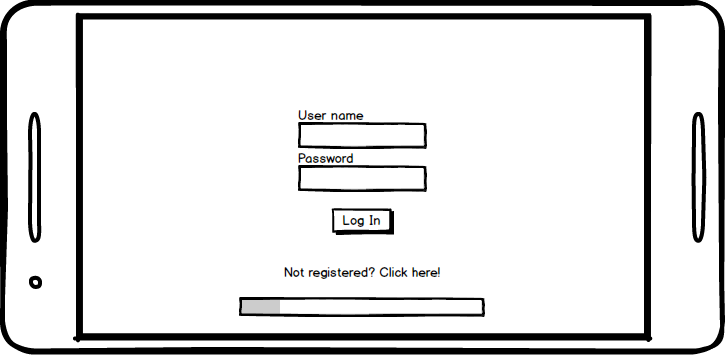
\includegraphics[width=10cm]{pics/Login.png}
				\captionof{figure}{Login-Screen Mockup} 
			\end{center}
			
			Falls sich der Benutzer bei NoRPG registrieren möchte, hat er die Möglichkeit dies in der App zu machen. Dazu klickt der Benutzer im Login-Screen auf den Register-Button. Anschließend öffnet sich der Register-Screen. Die Elemente sind im Tabellen Layout angeordnet, wodurch der Benutzer weiß, welche Daten in welches Feld eingetragen werden müssen. Die Registrierung ist notwendig, damit der Spielstand, somit der Fortschritt in einer Relation mit dem Benutzer steht. Zur weiteren Optimierung werden kurze Fehlermeldungen ausgegeben, damit ich der Benutzer weiß, in welchem Feld ein Fehler ist.
			
			\begin{center}
				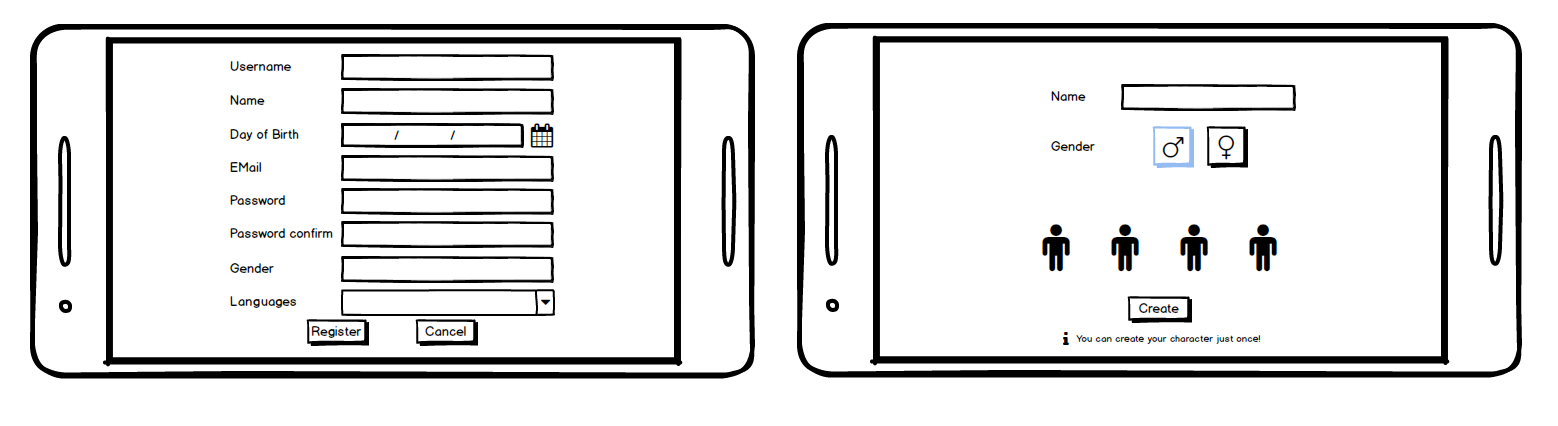
\includegraphics[width=\textwidth]{pics/Registerprozess.png}
				\captionof{figure}{Registerprozess: Registrierung und Create Character Mockup} 
			\end{center}
			
			Nach der Registrierung kann der Spieler einmalig seinen Charakter für den angelegten Account erstellen. Dazu bestimmt der Benutzer den Namen, das Geschlecht und das Aussehen des Charakters.
			
			NoRPG startet, nachdem alles geladen wurde und der Benutzer angemeldet ist. Das Spiele-Screen besteht aus der Spielewelt (Grafik) und dem Head-Up Display, kurz HUD. Das HUD ist eine Methode, mit der Informationen visuell als Teil der Benutzeroberfläche eines Spiels vermittelt werden. Während die Informationen, die auf dem HUD angezeigt werden, stark vom Spiel abhängen, gibt es viele Eigenschaften, die Spieler über viele Spiele erkennen. Die meisten von ihnen sind statisch auf dem Bildschirm, so dass sie während des Spiels sichtbar bleiben. 
			
			\begin{center}
				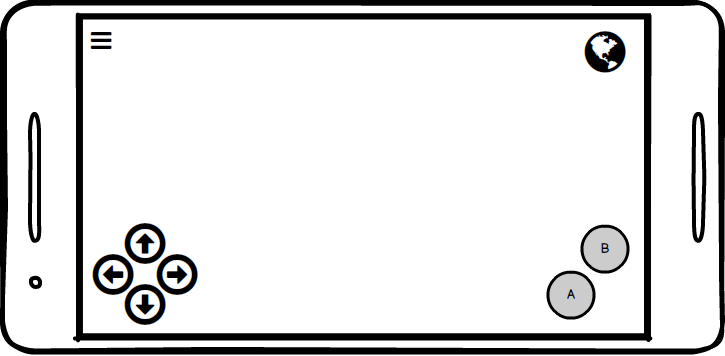
\includegraphics[width=10cm]{pics/HUD.png}
				\captionof{figure}{HUD Mockup} 
			\end{center}
			
			Das Mockup 3 enthält alle direkt sichtbaren HUD Elemente, die während des Spieles aktiv sind. Die Elemente sind an die Ecken gebunden, so befindeen sich beispielsweise die Pfeiltasten zur Bewegung des Charakters in der linken unteren Ecke des Bildschirms (siehe Graifk). Es sind so wenig Elemente wie möglich auf dem Bildschirm angeordnet und die verwendeten Symbole sind aus anderen bekannten Spielen und Konsolen übernommen und sind quasi ein Standard. Durch diese bekannte Anordnung der Elemente kann der User Informationen schneller verstehen und schneller reagieren. %vllt bisschen noch was zu dieser Anordnung labern
			
			Das Menü, welches sich in der oberen linken Ecke befindet, kann geöffnet werden. Dadurch wird das laufende Spiel pausiert und es werden weitere Optionen bzw. Interaktionen mit dem Spiel möglich. Diese HUD Elemente werden nur dann sichtbar, wenn der Spieler das Menü öffnet. Dadurch rückt das Spiel und die anderen Elemente in den Hintergrund. Das bedeutet nicht, dass die Elemente ausgeblendet werden, sondern dass der Benutzer diese Elemente nicht benutzen kann solange das Menü offen ist.
			
			\begin{center}
				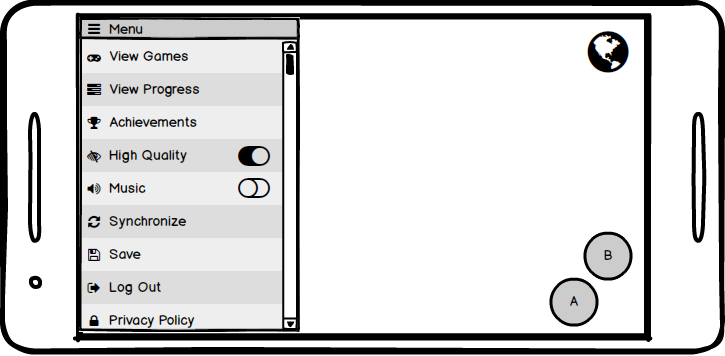
\includegraphics[width=10cm]{pics/Menu.png}
				\captionof{figure}{HUD offenes Menü Mockup} 
			\end{center}
			
			Einige der Menü-Elemente öffnen wiederum einen anderen Screen. Diese werden dann über das aktuelle Spiel geöffnet. Das Spiel befindet sich im Hintergrund und kann nicht gesehen bzw. angeklickt werden. Der neu geöffnete Screen muss erst geschlossen werden um das Spiel fortsetzen zu können. Ein Beispiel dafür ist der Fortschritt-Screen. Hier kann der Benutzer seinen Lern- bzw. Spielfortschritt betrachten.
			
			\begin{center}
				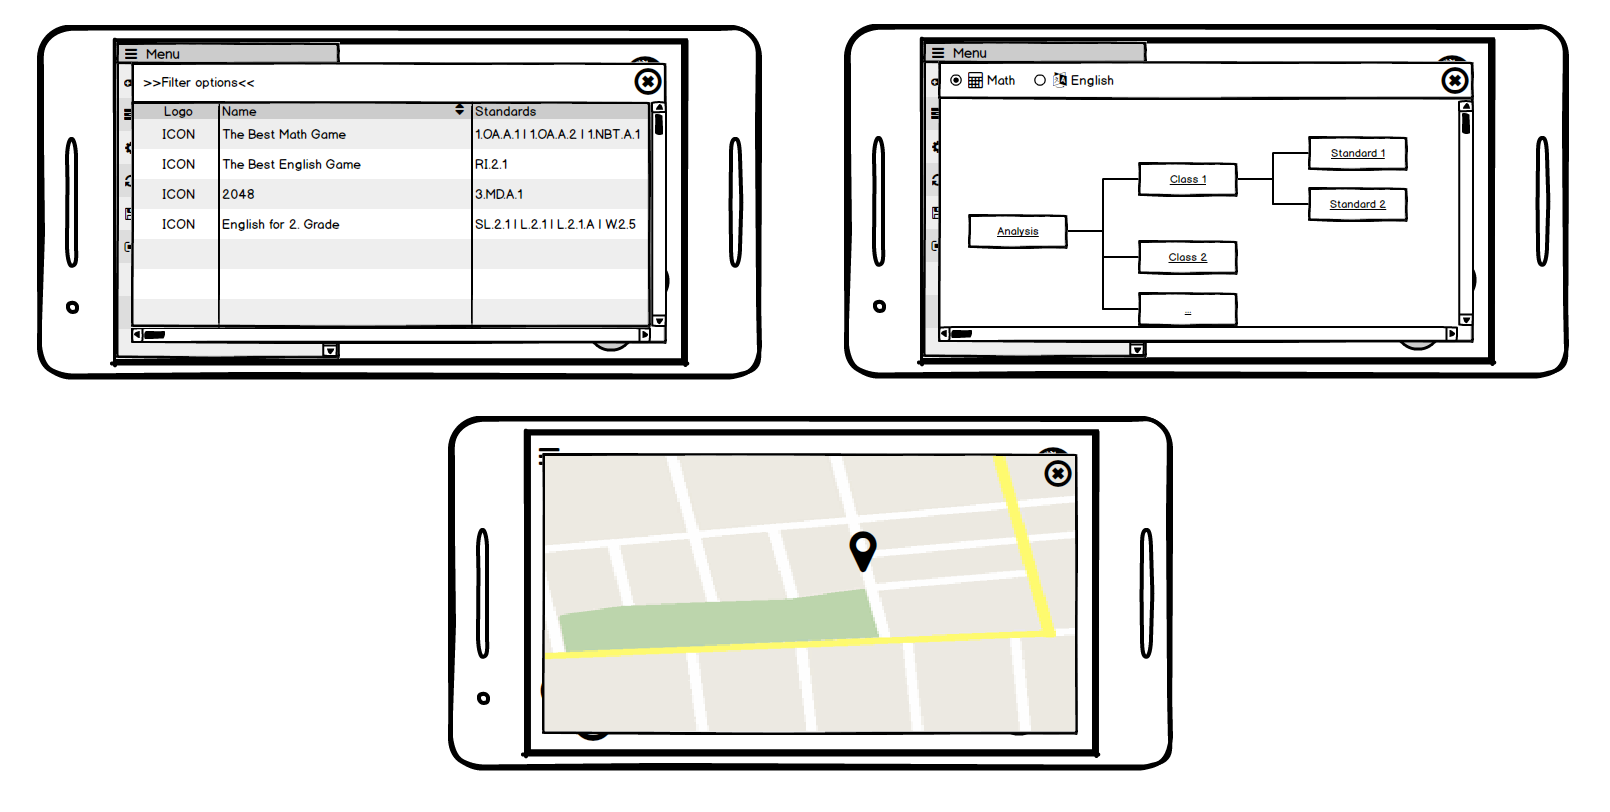
\includegraphics[width=\textwidth]{pics/NewWindows.png}
				\captionof{figure}{Spieleliste-, Fortschritt- und Karte-Fenster Mockup} 
			\end{center}
			
			Die Auflistung aller Screens würde den Rahmen dieser Arbeit überschreiten. Daher befinden sich die Mockups für die restlichen Screens im Anhang.
						
			%logische Eigenschaften:  required screen formats, page or window layouts, content of any reports or menus, or availability of programmable function keys
			
			%Aspekte Optimierung: comprise a list of do's and don'ts on how the system will appear to the user: long or short error messages
		
		\subsubsection{Hardwareschnittstellen}
			Die Hardwareschnittstellen spezifiziert die logischen Eigenschaften jeder Schnittstelle zwischen NoRPG und den Hardwarekomponenten des Systems. Die App hat eine  Hardwareschnittstelle mit dem Smartphone und seinen Komponenten.
			
			Ein Smartphone besteht aus sehr vielen Hardwarekomponenten. Jede einzelne Komponente wird benötigt, damit das Smartphone mit seinem kompletten Funktionsumfang funktioniert. Jedoch spielen einige Hardwarekomponenten eine besondere Rolle. Zu einem der Touchscreen eines Smartphones -> Toucheingaben für die Steuerung des Charakters, Interaktion mit dem Spiel, Menü, etc --> die einzige Benutzerschnittstelle
			
			WLAN-Adapter - verbindung mit dem Internet um mit dem Server zu kommunizieren
			
		\subsubsection{Softwareschnittstellen}
			This should specify the use of other required software products and interfaces with other application systems 
			
			Data mangement system, Google Play Store, 
			
			Software - Kommunikation mit GUI, kommunikation mit DB, ggf. logging

	\subsection{Funktionale Anforderungen}
		Use Cases dokumentieren Funktionalitäten eines Systems auf Basis von einfachen Modellen. In einem Use Case wird das nach außen sichtbare Verhalten eines Systems aus der Sicht der Nutzer beschrieben. Ein Nutzer kann hierbei eine Person, eine Rolle oder ein anderes System sein. Dieser Nutzer tritt als Akteur mit dem System in Interaktion, um ein bestimmtes Ziel zu erreichen. %quelle
		
		Use Cases verwenden Activity UML um anzuzeigen, wie der Benutzer vorgehen muss. Ein Aktivitätsdiagramm ist ein Verhaltensdiagramm der Unified Modeling Language (UML) und stellt die Vernetuzung von elementaren Aktionen und deren Verbindungen mit Kontroll- und Datenflüssen grafisch dar.
	
		\begin{center}
			
\includegraphics[width=10cm]{pics/OUCD.pdf}
			\captionof{figure}{Overall Use Case Diagramm} 
		\end{center}
		
		Das abgebildete System stellt die zu entwickelnde App für die User dar. Die App stellt die Graphische Oberfläche und somit die beschrieben Benutzerschnittstellen dar. Es sind nur die Funktionalitäten enthalten, die der Benutzer ausführen kann, also jene die über die Benutzerschnittstellen angesprochen werden können. Use Cases wie Login oder Registrierung sind im Overall Use Case Diagramm nicht enthalten, da diese im Vergleich zu anderen Use Cases primitiv sind. 
		
		Es werden nur die Use Cases des Players betrachtet, da die Use Cases des zweiten Benutzers, den Administratoren, zunächst nicht implementiert sondern nur entsprechende Vorkehrungen für die Implementierung getroffen werden.
	
		\subsubsection{Create character}
			Dieser Use Case beschreibt den Anwendungsfall, dass der Benutzer seinen Charakter erstellen möchte. Dieser Use Case wird pro Account genau einmal nach der Registrierung ausgeführt und zählt noch zum Prozess der Registrierung.
			
			Nach erfolgreicher Registrierung kann der Spieler seinen Charakter erstellen. Der User kann seinem Charakter einen Namen geben, das Geschlecht auswählen und anschließend das Aussehen bestimmen. Anschließend wird dem User der Hinweis angezeigt, dass es sich um eine einmalige Aktion handelt. Nachdem diese bestätigt wurde, wird der Charakter erstellt und gespeichert.
				
			\begin{center}
				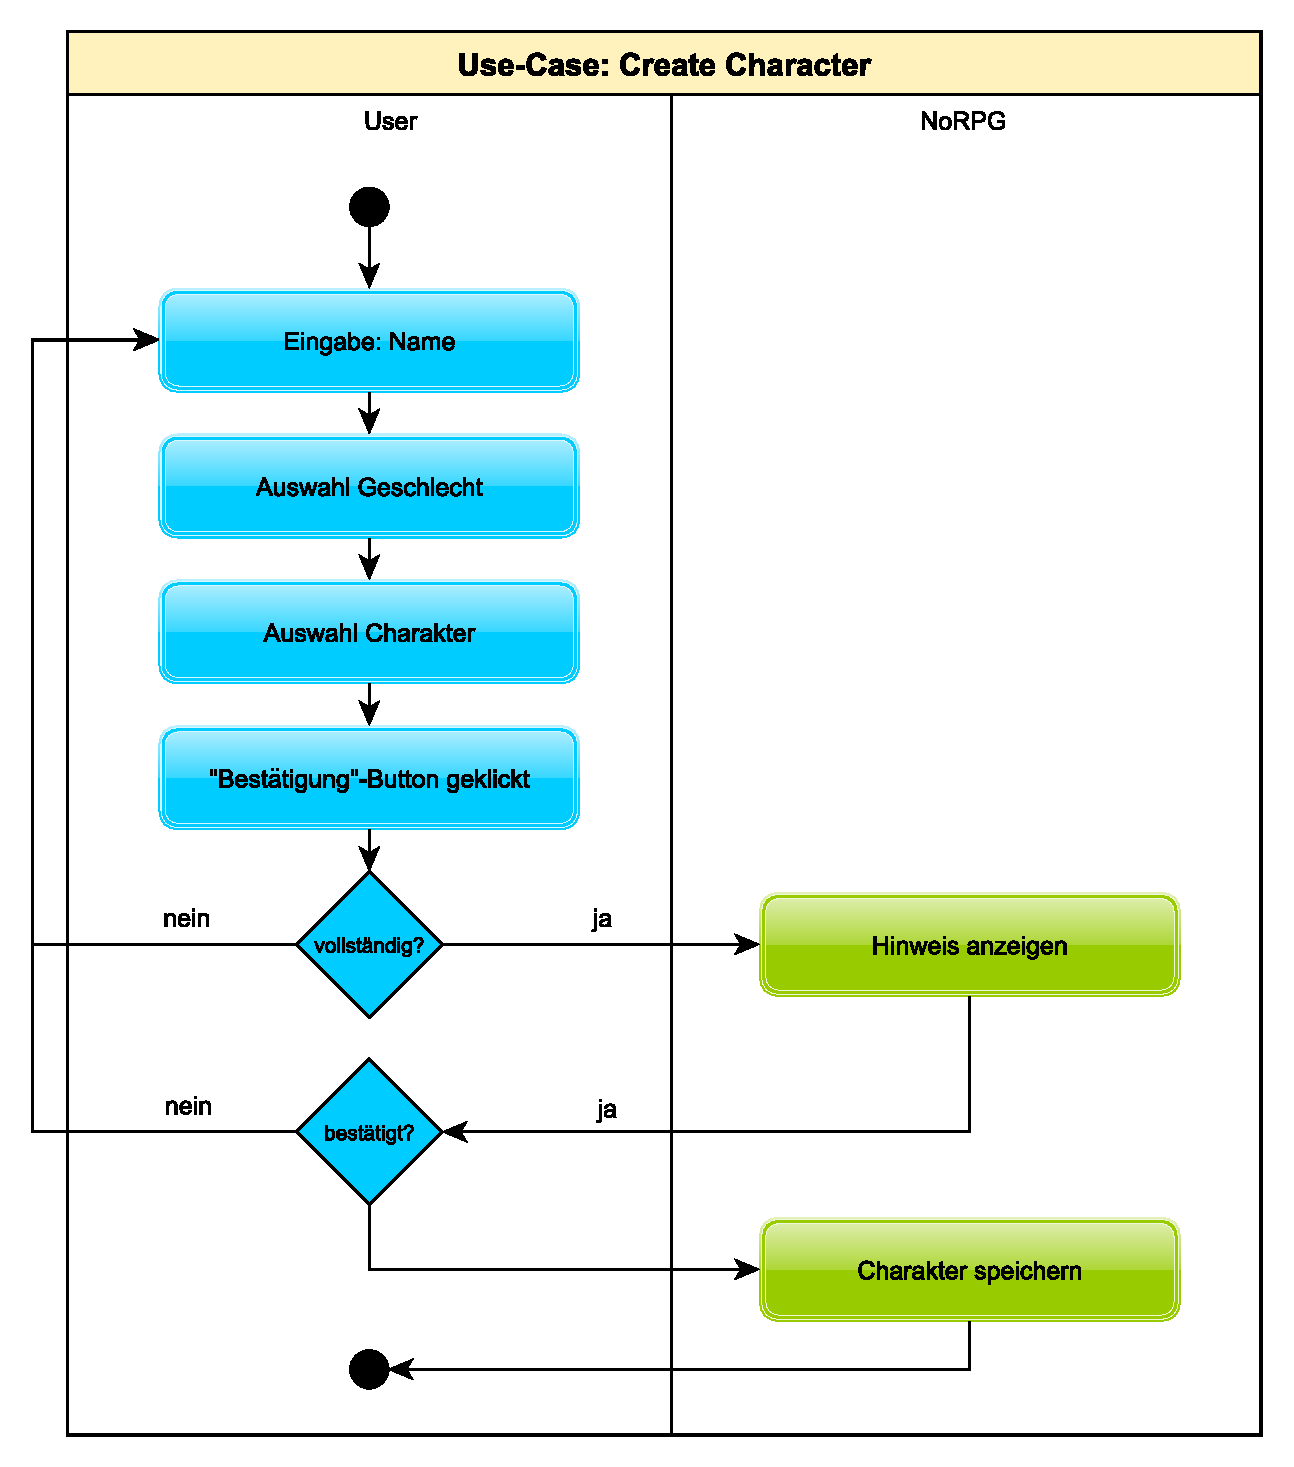
\includegraphics[width=10cm]{pics/CreateCharacter.pdf}
				\captionof{figure}{Create Character Activity UML} 
			\end{center}
	
			Bevor jedoch dieser Use Case ausgeführt werden kann, muss die Registrierung vollständig und erfolgreich abgeschlossen werden. Die Registrierung ist erfolgreich, wenn alle benötigte Daten eingetragen wurden und der Account noch nicht existiert. Für den gesamten Registrierungsprozess wird eine aktive Internetverbindung benötigt.
			
			Nach erfolgreicher Erstellung des Charakters, wird dieser in die Datenbank gespeichert und der User kann sich nun anmelden und in die Rolle seines Charakters schlüpfen.
			
		\subsubsection{Open map}
			Dieser Use Case beschreibt den Anwendungsfall, dass der Benutzer die Karte öffnet. Die Karte dient zur Orientierung der Welt und beinhaltet Symbole etc. um herauszufinden was so ist
			
			Ereignisablauf:	Benutzer öffnet Menü und klickt auf "Map" ...
	
			Vorbedingungen: Menü offen, Benutzer befindet sich nicht in einer NPC Interaktion
			
			Nachbedingungen: Eine Karte von der aktuellen Welt wird geöffnet
	
		\subsubsection{Show games}
			Dieser Use Case beschreibt den Anwendungsfall: Liste der gespielten und heruntergeladneen Spiele wird angezeigt. Zuordnung zu den Standards. Aus NoRPG das Spiel starten können.
			
			Ereignisablauf: Benuter öffnet Menü und klickt auf "Games" ...

			Vorbedingungen: Menü offen, Benutzer befindet sich nicht in einer NPC interaktion
			
			Nachbedingungen: Eine Liste wird angezeigt
	
		\subsubsection{View progress}
			Dieser Use Case beschreibt den Anwendungsfall, dass der Benutzer 
			
			Ereignisablauf
	
			Vorbedingungen
			
			Nachbedingungen
	
		\subsubsection{Settings}
			Dieser Use Case beschreibt den Anwendungsfall, dass der Benutzer 
			
			Ereignisablauf
	
			Vorbedingungen
			
			{Nachbedingungen
	
		\subsubsection{Synchronize}
			Dieser Use Case beschreibt den Anwendungsfall, dass der Benutzer 
			
			Ereignisablauf
	
			Vorbedingungen
			
			Nachbedingungen
	
		\subsubsection{Save local}
			Dieser Use Case beschreibt den Anwendungsfall, dass der Benutzer 
			
			Ereignisablauf
	
			Vorbedingungen
			
			Nachbedingungen
		
		\subsubsection{Character control}
			Dieser Use Case beschreibt den Anwendungsfall, dass der Spieler seinen Charakter in NoRPG durch die Spielwelt kontrolliert.
			
			Ereignisablauf
			
			Vorbedingungen: Spieler befindet sich im Spiel (nicht loading screen und menü ist geschlossen)
			
			Nachbedingungen: Charakter bewegt sich, bestätigt oder lehnt ab
	
		\subsubsection{game interaction}
			Dieser Use Case beschreibt den Anwendungsfall, dass der Benutzer sich in einer Interaktion mit einem NPC befindet. NPC bedeutet Non-Player Charakter und stellt die programmierten Charaktere dar (Unterhaltungen mit NPC, Storytelling)
			
			Ereignisablauf
			
			Vorbedingungen: Spieler befindet sich im Spiel (nicht loading screen und menü ist geschlossen)
			
			Nachbedingungen: Charakter bewegt sich, bestätigt oder lehnt ab
				
		%\begin{itemize}
		%	\item{Die Interaktion mit NPC's starten eine Unterhaltung, wodurch der Spieler mehr über das Spiel erfahren kann.}
		%	\item{Die Interaktion mit einer Verschlossenen Truhe zeigt die Lernspiele, die gespielt werden müssen um die Truhe öffnen zu können.}
		%	\item{Die Interaktion mit einer freigespielten True, ermöglicht dem Spieler die Truhe zu öffnen.}
		%	\item{Die Interaktion mit Collectables, die durch das Suchen/Reisen gefunden werden können, sammelt diese.}
		%	\item{Die Interaktion mit der Umwelt (Tiere, Bäume, etc.) startet keine Aktion.}
		%\end{itemize}
	
	\subsection{Performanz Anforderungen}
		This subsection should specify both the static and the dynamic numerical requirements placed on the software or on human interaction with the software as a whole. Static numerical requirements may include the following
		
		The number of terminals to be supported, The number of simultaneous users to be supported, Amount and type of information to be handled
		
	\subsection{Datenbank Anforderungen}
		This should specify the logical requirements for any information that is to be placed into a database. This may include the following:
		
		Types of information used by various functions
		
		Frequency of use
		
		Accessing capabilities
		
		Data entities and their relationships
		
		Integrity constraints
		
		Data retention requirements.
	
	\subsection{Entwurfsbeschränkungen}
		This should specify design constraints that can be imposed by other standards, hardware limitations, etc.
		
		Standards compliance: This subsection should specify the requirements derived from existing standards or regulations. They may include the following: 
		
		Report format, Data naming, Accounting procedures and Audit tracing.
		
		Als Maßstab werden dabei die Hardware des Smartphones Samsung Galaxy S4 genommen. Das Samsung Galaxy S4 kostet ungefähr 250 Euro\footnote{Stand 04.01.2017 \url{https://www.amazon.de/Samsung-Smartphone-Touch-Display-Speicher-Android-Schwarz/dp/B00BTCE2M0}} und hat das Betriebssystem Android 5.0 Lollipop vorinstalliert und besitzt ausreichend gute Hardwarekomponenten. Die Auflösung des Displays mit 1080 x 1920 Pixel ist ausreichend, die 2 GByte Arbeitsspeicher sind notwendig und die 16 GByte interner Speicher sind ausreichend. Bei dem Prozessor handelt es sich um ein Qualcomm Snapdragon 600, mit vier Kernen und einer 32-bit Architektur\footnote{für mehr Informationen: \url{http://www.samsung.com/de/consumer/mobile-devices/smartphones/galaxy-s/GT-I9506ZKADTM}}.
	
	\subsection{Benutzerfreundlichkeit}
		Das Ziel der Benutzerfreundlichkeit ist eine hohe Ergonomie. Die Software-Ergonomie bezeichnet die Anpassung an die kognitiven und physischen Fähigkeiten bzw. Eigenschaften des Benutzers, also seine Möglichkeiten zur Verarbeitung von komplexen Informationen aber auch die Anpassung softwaregesteuerten Merkmale der Darstellung, wie Farben und Schriftgröße.
		
		Damit die Benutzeroberfläche freundlich für den Benutzer ist, muss sie in das Profil des Benutzers passen. Da NoRPG sich grundsätzlich an Kinder richtet muss die Bedienung und Gestaltung der App kindgerecht sein. 
		
		Zur kindgerechten Gestaltung gehört auch, dass keine In-App-Käufe angeboten werden. Keine Werbung. Wenig Berechtigungen bei der Installation (nur das notwendigste)
		Keine Verlinkungen zu Social Media oder ähnlichem. Nur wenn notwendig, an die Spiele von Google Play Store verlinken \footnote{\url{http://www.wir-machen-kinderseiten.de/blog/was-macht-eine-gute-kinder-app-aus}}
		
		Kindgerecht: Einfach, simpel, 
		
		Leserlichkeit
		
		Entdecken: Farbenfroh, animiert --> Wahrnehmung und Aufmerksamkeit erhöhen
		
		Bsp: sichtbares Steuerkreuz anstatt Ziehfunktion wie bei anderen RPGs (vielleicht ein Bild hier um den Unterschied zu verdeutlichen)
		--> Navigation soll schnell erkennbar und nachvollziehbar sein
		
		Durchführen von Usability-Tests
		
		Finally, while you should be focusing on children users, don’t forget about adults! I’m talking about parents, guardians, teachers, and anyone who may interact with the app. What role do adults play in the app? Are they an equal play partner, playing alongside children? Are they assisting or supervising play? Can they troubleshoot when something goes wrong? Or maybe they are a separate type of user to consider altogether. For example, teachers may need to log in to a separate section of the app to check each student’s progress. \footnote{\url{https://www.smashingmagazine.com/2016/01/designing-apps-for-kids-is-not-childs-play/}}
		
		Wendy B. von Intel beschreibt in Ihrem Artikel "Apps for Kids: Basic Usability Guidelines"\footnote{\url{https://software.intel.com/en-us/blogs/2013/01/23/apps-for-kids-basic-usability-guidelines}} vier Prinzipien für kindgerechte Apps
		\begin{enumerate}
			\item{Freedom: The ability to move within the app within a controlled environment}
			\item{Comfort: Stimulation, but not too much stimulation. Audio input, but not too much. It’s a balancing act. Varied levels of stimulation are definitely needed, but there’s a fine line between stimulation and just noise for the sake of noise.}
			\item{Confidence: Kids – just like us adults – need to feel that they are competent. They want to have confidence in what they are doing.}
			\item{Control: Children want to feel that they are accomplishing something when they are interacting within an app. Goals are met, decisions are being made.}
		\end{enumerate}

	\subsection{Zuverlässigkeit}
		%This should specify the factors required to establish the required reliability of the software system at time of delivery.
		Alle implementierte Funktionen sollten zur Auslieferung korrekt und zuverlässig funktionieren. Dazu zählt auch, dass die Funktionen in vertretbaren Zeiten terminieren. Beispielsweise sollte die Anmeldung funktionieren, wenn der Spieler registriert ist und die richtigen Benutzerdaten eingegeben hat, oder die Benutzereingaben für die Charaktersteuerung sollen korrekt interpretiert werden.
		
		Eine besondere Wichtigkeit hat die Implementierung der in Kapitel 2 beschriebenen Common Core State Standards. Diese sind wichtig für die Reihenfolge der spielbaren Lernspiele, damit ein Spieler mit einem Skilllevel der ersten Klasse in Geometrie keine Lernspiele für die fünfte Klasse angezeigt kriegt. Erst dadurch wird gewährleistet und kann sichergestellt werden, dass der Spieler die Lerninhalte korrekt vermittelt kriegt.
	
	\subsection{Verfügbarkeit}
		%This should specify the factors required to guarantee a defined availability level for the entire system such as checkpoint, recovery, and restart. 
		
		Da bei jeder App eine lokale Datenbank mit vorhanden ist, muss der Server nicht ganze Zeit verfügbar sein. Das gilt jedoch nur für die Benutzer, die NoRPG schon heruntergeladen und sich registriert sowie angemeldet haben. Wenn diese Bedingungen erfüllt sind, wird der ganze Fortschritt lokal gespeichert werden und kann mit dem Server manuell oder vor dem Ausloggen automatisch synchronisiert werden, muss es allerdings nicht. Denn der Server ist da, falls der User sich an einem anderen Gerät anmelden möchte, dass der Spielstand dort gleich ist. 
		
		System Availability: MUST: 98\%, PLAN: 99\% und WISH: 100\%
		
		Server Availability: MUST: 80\%, PLAN: 99\% und WISH: 100\%
		
		Internet Connection: Die App sollte mit dem Internet verbunden sein, jedoch muss es nicht
		
	\subsection{Sicherheit}
		Bei Sicherheit wird zwischen zwei unterschiedlichen Typen unterschieden: Security und Safety. Security ist der Schutz vor absichtlichen Bedrohungen, wenn ein Angreifer absichtlich das Systems angreift. Im Gegensatz dazu ist Safety der Schutz vor unbeabsichtigten Bedrohungen, wenn der Benutzer durch Zufall die Sicherheitsmechanismen umgeht indem er etwas nicht beabsichtigtes ausführt.
		
		Die Kommunikation mit dem Server und mit der lokalen eingebetteten Datenbank müssen verschlüsselt werden, damit die Credentials bei den Anmeldung oder bei der Registrierung nicht mitgelesen werden können. Des Weiteren müssen die Daten auf der lokalen Datenbank validiert werden, bevor der Server synchronisiert wird, denn es wird unter anderem auch der Spielfortschritt der Benutzer synchronisiert. Die Veränderung des Spielfortschritts wird als Schummeln bzw. Cheaten behandelt.
		
		Die Anmeldung bzw. Registrierung ist notwendig, um NoRPG spielen zu können. Deswegen müssen die Accounts der Benutzer verschlüsselt gespeichert werden und die Passwörter dürfen bei der Anmeldung nur mittels One-Way-Functions vergleichen werden. Nicht registrierte bzw. unautorisierte Benutzer erlangen keinen Zugriff auf das System.
		
		Die gespeicherte Daten dürfen an andere Tools nur anonymisiert weitergegeben werden, für beispielsweise Analysezwecke. Diese Kommunikation mit anderen System oder Applikationen darf nur verschlüsselt geschehen.
		
	\subsection{Wartbarkeit}
		Der Code von NoRPG sollte so geschrieben werden, dass der Code die Umsetzung neuer Funktionen begünstigt. Deshalb sollte die Komplexität des Codes so gering wie möglich gehalten werden, indem entsprechende Methoden wie das Model-View-Controller Pattern umgesetzt werden. Des Weiteren sollte das System von NoRPG Schnittstellen jeglicher Art anbieten, um das System durch weitere Komponenten wie ein Web-Tool für Administratoren zu erweitern.
		
		Neben der Erweiterbarkeit sollte NoRPG für Fehlerfälle eine Testumgebung anbieten, um das Testen der Anwendung auf unterschiedliche Funktionen zu ermöglichen und gegebenenfalls Fehler wiederholen und simulieren zu können.
		
	\subsection{Portabilität}
		Die App NoRPG ist zunächst nur für Android geplant. Andere Betriebssysteme, wie Windows Phone von Microsoft oder iOS von Apple, sind vorerst nicht vorgesehen. 
		
		Bei der vorhanden Breite an Varianten von Android-Smartphones ist sehr wichtig, dass die Portabilität innerhalb von Android Smartphones gewährleistet wird. Neben bekannten Smartphoneherstellern wie Samsung, LG oder HTC gibt es zahlreiche weitere Hersteller die auf das Android Betriebssystem setzen. Jeder Hersteller hat dabei eine große Palette an Smartphone-Modellen, wie bei Samsung die Samsung Galaxy S-Reihe, welches aktuell in der siebten Genration erhältlich ist\footnote{Vgl. \url{http://www.computerbild.de/artikel/cb-News-Handy-Samsung-Galaxy-S-S2-S3-S4-S5-S6-S7-11332036.html}}, oder die Samsung Galaxy Note-Reihe. Die App NoRPG muss auf allen Android-Smartphones funktionieren, solange diese die Mindestanforderungen an Software und Hardware erfüllen. Dabei muss sich die App beispielsweise an die Auflösung oder XXX anpassen.
		
		Die Portabilität beschreibt nicht nur die technische Sicht sondern auch in welchen Ländern und in welchen Sprachen NoRPG verfügbar sein wird. Der Release findet in allen Ländern statt, in denen der Google Play Store verfügbar ist. Zunächst wird NoRPG nur in Englisch verfügbar sein, welches jedoch kein weiteres Problem darstellt.